% *********************************************************************
% © 2021–2026 Jeremy Sylvestre
%
% Permission is granted to copy, distribute and/or modify this document
% under the terms of the GNU Free Documentation License, Version 1.3 or
% any later version published by the Free Software Foundation; with no
% Invariant Sections, no Front-Cover Texts, and no Back-Cover Texts. A
% copy of the license is included in the appendix entitled “GNU Free
% Documentation License” that appears in the output document of this
% PreTeXt source code. All trademarks™ are the registered® marks of
% their respective owners.
%
% *********************************************************************

\newcommand*{\xmin}{-0.1}
\newcommand*{\xmax}{3}
\newcommand*{\ymin}{-1.25}
\newcommand*{\ymax}{4}
\newcommand*{\func}{\x * \x * \x * \x / 4 - 3 * \x * \x * \x / 2 + 11 * \x * \x / 8 + 29 * \x / 8 - 63 / 64}

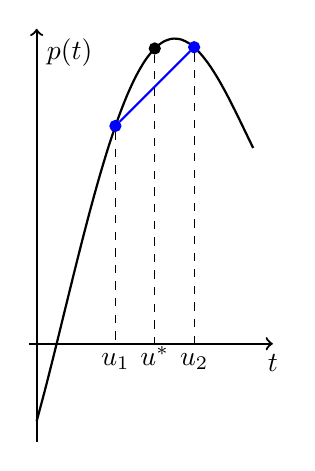
\begin{tikzpicture}
[
	closedpt/.style={circle,draw,fill,inner sep=0pt,minimum size=4pt},
	openpt/.style={circle,draw,inner sep=0pt,minimum size=4pt},
%	xscale=2,
	yscale=1
]


	% example graph
	\draw[thick, domain=0:2.75, smooth, thick] plot (\x,{\func});

	% axes
	\draw[->,thick] (\xmin,0) -- (\xmax,0) node[below] {$t$};
	\draw[->,thick] (0,\ymin) -- (0,\ymax) node[below right] {$p(t)$};

	\node[closedpt,blue] at (1,2.766) (qlefthalf) {};
	\node[closedpt] at (1.5,3.75) (qcentre) {};
	\node[closedpt,blue] at (2,3.766) (qrighthalf) {};

	\draw[blue, thick] (qlefthalf) -- (qrighthalf);

	\node[below] at (1.5,0.09) (tcentre) {$u^\ast$};

	\draw[dashed] (qcentre) -- (1.5,0);

	\draw[dashed] (qlefthalf) -- (1,0) node[below] {$u_1$};
	\draw[dashed] (qrighthalf) -- (2,0) node[below] {$u_2$};

\end{tikzpicture}
